\documentclass{article}
\usepackage[utf8]{vietnam}
\usepackage[11pt]{extsizes}
\usepackage{amsmath,amsfonts,amsthm}
\usepackage{geometry}
\usepackage{graphicx}
\usepackage{float}
 \geometry{
 a4paper,
 total={170mm,257mm},
 left=20mm,
 top=20mm,
}
\usepackage{enumitem} 
\title{Ontology và TOPSIS}
\begin{document}
\maketitle
\section{Module sử dụng Ontology tìm thuốc cho bệnh nhân}
\subsection{Định nghĩa Ontology}
\begin{itemize}
    \item[--] Cụm từ "Ontology" là một từ ghép trong tiếng Hy Lạp được cấu thành từ
hai chữ "onto" nghĩa là sự tồn tại và "logy" nghĩa là khoa học. Trong triết học, "Ontology"
là ngành khoa học nghiên cứu về bản chất sự tồn tại của các thực thể và cách chúng liên quan với nhau.
    \item[--] Tương tự, trong khoa học máy tính, "Ontology" là mô hình dữ liệu biểu diễn một lĩnh vực cụ thể
thông qua các khái niệm, mối quan hệ và các quy tắc giữa chúng.
\end{itemize}
\subsection{Cấu trúc của Ontology}
\begin{itemize}
    \item[--] Individuals (cá thể): là thành phần cơ bản và hạt nhân nhất của ontology.
    \item[--] Classes (lớp): là tập hợp của các lớp con hoặc các cá thể có đặc điểm chung.
    \item[--] Properties (thuộc tính): là thuộc tính mà cá thể sở hữu.
    \item[--] Relations (quan hệ): là mối quan hệ giữa các đối tượng được diễn tả thông qua các thuộc tính của chúng.
\end{itemize}
Ví dụ về cấu trúc của Ontology:
\begin{figure}[ht]
    \centering
    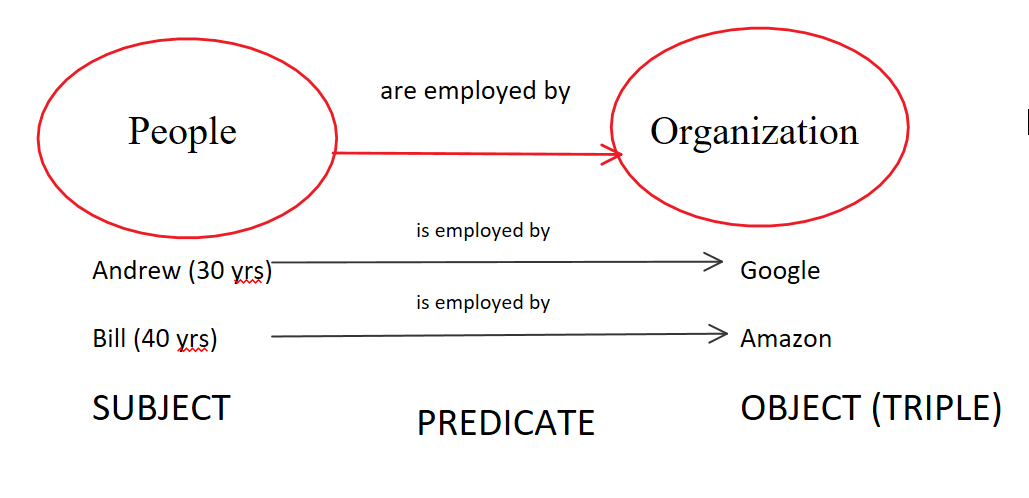
\includegraphics[width=0.8\textwidth]{ontology.png}
    \caption{Cấu trúc Ontology}
    \label{dongco}
\end{figure}
\newpage
\begin{enumerate}
    \item Classes: trong hình vẽ này ta thấy có hai class là "People" và "Organization".
    \item Individuals: ta thấy có 4 individual được thể hiện trong hình minh họa là "Andrew", "Bill", "Google" và "Amazon".
    \item Properties: ta dễ dàng thấy property của Andrew là 30 years old còn Bill là 40 years old.
    \item Relation: ta thấy mối quan hệ giữa Andrew và Google, cũng như Bill và Amazon hay mọi người và tổ chức đó là "được tuyển dụng".
\end{enumerate}
Dễ thấy từ hình vẽ mô tả trên, ta có thể thấy Ontology chứa dữ liệu dưới dạng bộ ba (triple) và thể hiện cấu trúc Subject-Predicate-Object rất rõ ràng.
\subsection{Sử dụng Ontology để tìm thuốc cho bệnh nhân}
    1. Sử dụng phần mềm Protege để tạo Ontology:
    \begin{figure}[H]
        \centering
        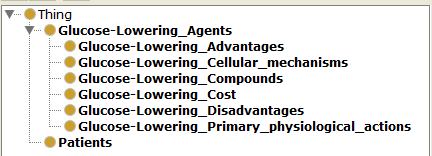
\includegraphics[width=0.8\textwidth]{o1.png}
        \caption{Class và các subclass sử dụng trong Ontology}
        \label{dongco}
    \end{figure}
 \begin{itemize}
    \item Glucose-LoweringAgents: class này thể hiện các tác nhân giúp giảm đường huyết qua các loại thuốc MET, SU, GLP-1,...
    \item Glucose-LoweringAdvantages: subclass này thể hiện lợi ích của các loại thuốc.
    \item Glucose-LoweringDisadvanges: subclass này thể hiện hạn chế của các loại thuốc
 \end{itemize}
 \begin{figure}[H]
    \centering
    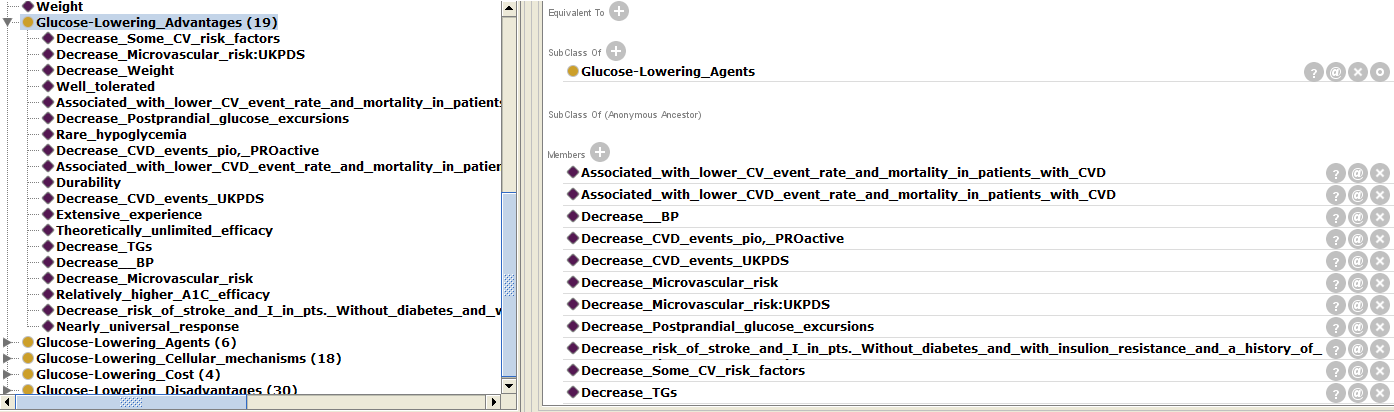
\includegraphics[width=0.8\textwidth]{o2.png}
    \caption{Subclass Glucose-LoweringAdvantages}
    \label{dongco}
\end{figure}
\begin{figure}[H]
    \centering
    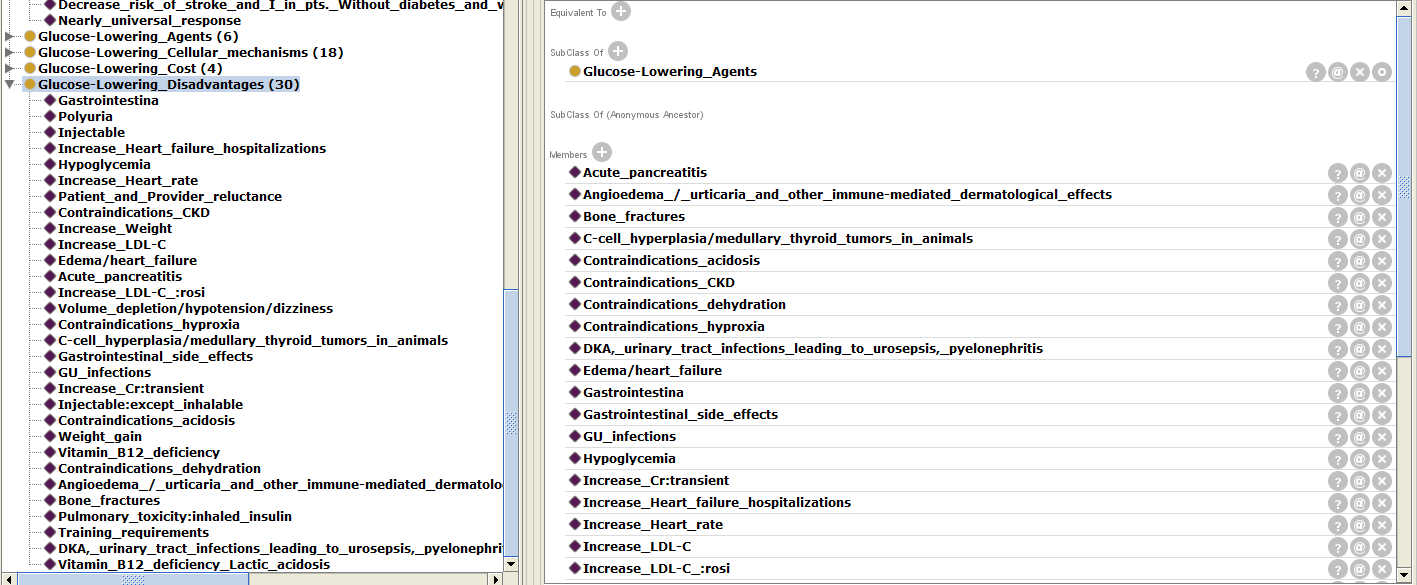
\includegraphics[width=0.8\textwidth]{o3.png}
    \caption{Subclass Glucose-LoweringDisadvanges}
    \label{dongco}
\end{figure}
\begin{figure}[H]
    \centering
    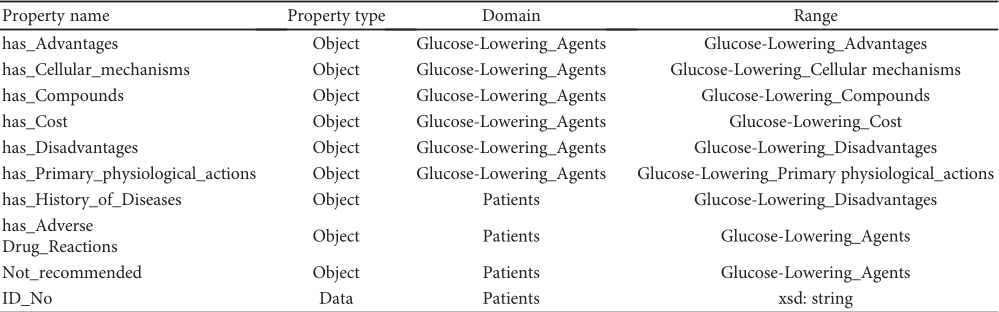
\includegraphics[width=0.8\textwidth]{o4.png}
    \caption{Các relation trong Ontology}
    \label{dongco}
\end{figure}
\begin{figure}[H]
    \centering
    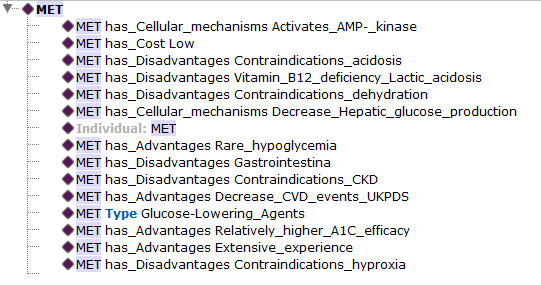
\includegraphics[width=0.8\textwidth]{o5.png}
    \caption{Thông tin về thuốc MET}
    \label{dongco}
\end{figure}
2. Sử dụng SPARQL Query để truy vấn data trong Ontology:
\begin{enumerate}
    \item Cấu trúc cơ bản của SPARQL: \begin{itemize}
        \item PREFIX: định nghĩa các tiền tố URI
        \item SELECT: xác định biến truy vấn
        \item WHERE: định nghĩa điều kiện lọc dữ liệu
    \end{itemize}
Ví dụ ta cần lấy thông tin về những cá thể thuộc class Person và tên của họ từ một dataset:
\begin{verbatim}
PREFIX ex: <http://example.org/>
SELECT ?person ?name
WHERE {
  ?person a ex:Person. \\Tìm tất cả các cá thể kiểu "person"
  ?person ex:hasName ?name. \\Tìm tên của từng cá thể qua thuộc tính hasName
}
    \end{verbatim}
    \item Giải thích: \begin{enumerate}
        \item PREFIX: Quy ước đường dẫn rút gọn tới địa chỉ triển khai Ontology là ex.
        \item SELECT: Xác định kết quả trả về của truy vấn cho hai biến ?person và ?name.
        \item WHERE: Xác định cách các biến và mối quan hệ giữa chúng được lấy ra từ data.
    \end{enumerate}
\end{enumerate}
Hệ thống hỗ trợ ra quyết định cho bệnh nhân tiểu đường sẽ dựa vào tiền sử của bệnh nhân, truy vấn xem tiền sử này liên quan
đến tác dụng phụ của các loại thuốc nào để loại bỏ chúng ra khỏi danh sách khuyến nghị cho bệnh nhân.
\section{Module xếp hạng thuốc tiểu đường sử dụng TOPSIS}
Sau khi đã tìm được thuốc phù hợp, việc tiếp theo ta cần làm là LOẠI BỎ các nhóm thuốc không phù hợp và XẾP HẠNG nhóm thuốc còn lại để tìm ra lựa chọn tối ưu nhất cho bệnh nhân.
\\ Chúng ta sẽ phân tích ví dụ sau: Giả sử có một bệnh nhân mẫn cảm với GLP-1 và có tiền sử bệnh increasing LDL-C, Edema và một bảng thống kê rủi ro thuốc kèm chi phí.
\begin{figure}[H]
    \centering
    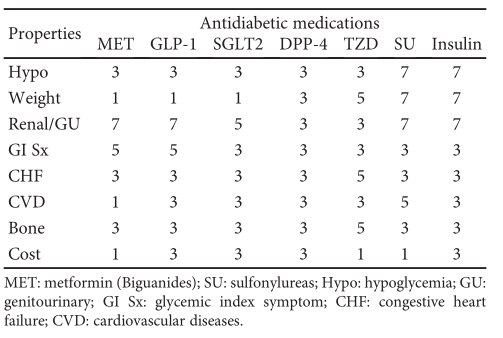
\includegraphics[width=0.8\textwidth]{o6.png}
    \caption{Rủi ro thuốc và chi phí}
    \label{dongco}
\end{figure}
Sau khi sử dụng Ontology, ta đã LOẠI BỎ được 3 loại thuốc không phù hợp vơi bệnh nhân là GLP-1, TDZ và SGLT2, ta sẽ
sắp xếp thứ tự ưu tiên của 4 loại thuốc sau đây:
\begin{figure}[H]
    \centering
    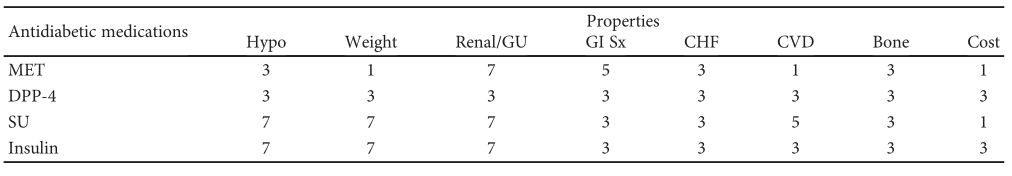
\includegraphics[width=0.8\textwidth]{o7.png}
    \caption{Danh sách chưa được sắp xếp}
    \label{dongco}
\end{figure}
Bước 1: Xây dựng ma trận quyết định
\begin{figure}[H]
    \centering
    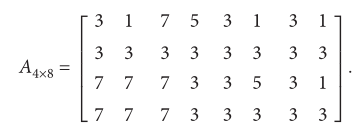
\includegraphics[width=0.8\textwidth]{o8.png}
    \caption{Ma trận quyết định}
    \label{dongco}
\end{figure}
Bước 2: Chuẩn hóa ma trận quyết định
\begin{figure}[H]
    \centering
    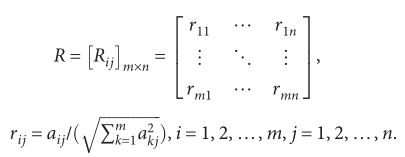
\includegraphics[width=0.8\textwidth]{o9.png}
    \caption{Chuẩn hóa ma trận quyết định}
    \label{dongco}
\end{figure}
\begin{figure}[H]
    \centering
    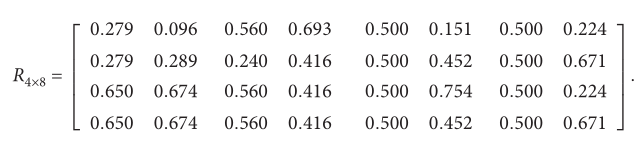
\includegraphics[width=0.8\textwidth]{o10.png}
    \caption{Kết quả}
    \label{dongco}
\end{figure}
Bước 3: Xác định trọng số của các thuộc tính và chi phí (Hypo, Weight, Cost,...):
\begin{figure}[H]
    \centering
    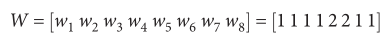
\includegraphics[width=0.8\textwidth]{o11.png}
    \caption{Ma trận trọng số}
    \label{dongco}
\end{figure}
Bước 4: Xây dựng ma trận chuẩn hóa trọng số
\begin{figure}[H]
    \centering
    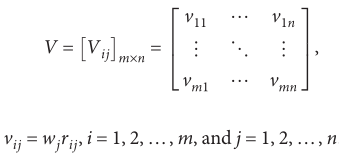
\includegraphics[width=0.8\textwidth]{o12.png}
    \caption{Ma trận chuẩn hóa trọng số}
    \label{dongco}
\end{figure}
\begin{figure}[H]
    \centering
    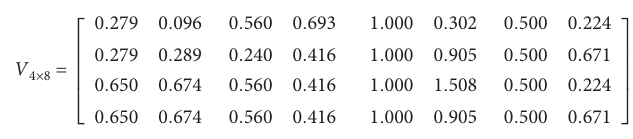
\includegraphics[width=0.8\textwidth]{o13.png}
    \caption{Kết quả}
    \label{dongco}
\end{figure}
Bước 5: Xác định các giải pháp lý tưởng và tiêu cực:
\begin{figure}[H]
    \centering
    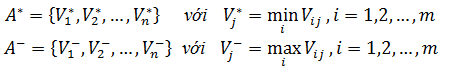
\includegraphics[width=0.8\textwidth]{o15.png}
    \caption{Phương pháp}
    \label{dongco}
\end{figure}
\begin{figure}[H]
    \centering
    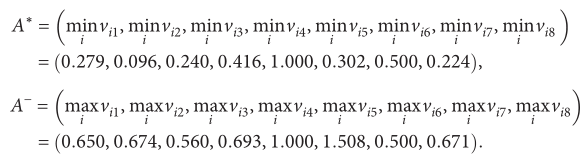
\includegraphics[width=0.8\textwidth]{o16.png}
    \caption{Kết quả}
    \label{dongco}
\end{figure}
Bước 6: Tính toán khoảng cách cho từng giải pháp:
\begin{figure}[H]
    \centering
    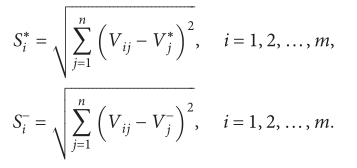
\includegraphics[width=0.8\textwidth]{o17.png}
    \caption{Phương pháp}
    \label{dongco}
\end{figure}
\begin{figure}[H]
    \centering
    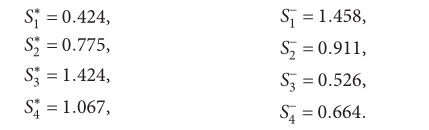
\includegraphics[width=0.8\textwidth]{o18.png}
    \caption{Kết quả}
    \label{dongco}
\end{figure}
Bước 7: Tính độ gần tương đối với mỗi phương pháp
\begin{figure}[H]
    \centering
    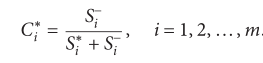
\includegraphics[width=0.8\textwidth]{o19.png}
    \caption{Phương pháp}
    \label{dongco}
\end{figure}
\begin{figure}[H]
    \centering
    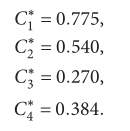
\includegraphics[width=0.8\textwidth]{o20.png}
    \caption{Kết quả}
    \label{dongco}
\end{figure}
Vậy ta kết luận phương án thuốc được sử dụng ưu tiên lần lượt là MET > DPP-4 > SU > Insulin
\end{document}